\documentclass{article}
\usepackage{amsmath}
\usepackage{amssymb}
\usepackage{tikz}
\usetikzlibrary{arrows,positioning}

\title{Mediation Analysis: Gene $\rightarrow$ Signature $\rightarrow$ Disease}
\author{}
\date{}

\begin{document}

\maketitle

\section{Mathematical Framework}

We test if genetic effects on disease are \textbf{mediated through signatures}.

\subsection{Pathway Model}

\begin{center}
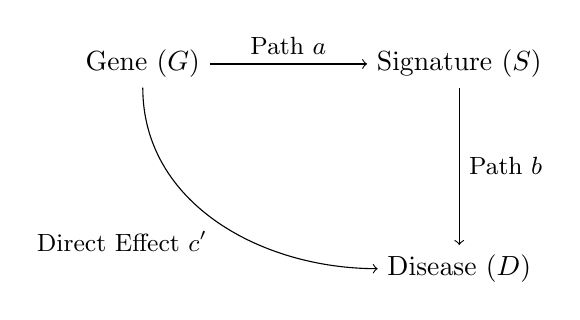
\begin{tikzpicture}[node distance=2cm, auto]
    \node (G) {Gene $(G)$};
    \node [right=of G] (S) {Signature $(S)$};
    \node [below=of S] (D) {Disease $(D)$};
    
    \draw[->] (G) -- node[above] {\small Path $a$} (S);
    \draw[->] (S) -- node[right] {\small Path $b$} (D);
    \draw[->] (G) to[out=270,in=180] node[below left] {\small Direct Effect $c'$} (D);
\end{tikzpicture}
\end{center}

Where:
\begin{itemize}
    \item \textbf{$G$}: Rare variant burden (gene-level)
    \item \textbf{$S$}: Signature loading ($\theta$, individual-level)
    \item \textbf{$D$}: Disease phenotype (binary, 0/1)
\end{itemize}

\section{Step 1: Total Effect (Gene $\rightarrow$ Disease)}

\textbf{Model:}
\begin{equation}
\text{logit}(P(D=1 \mid G)) = \beta_0 + c \cdot G
\end{equation}

\textbf{Interpretation:}
\begin{itemize}
    \item $c$ = Total effect of Gene on Disease (log odds ratio)
    \item If $c > 0$: Higher burden $\rightarrow$ Higher disease risk
    \item If $c = 0$: No association
\end{itemize}

\section{Step 2: Path $a$ (Gene $\rightarrow$ Signature)}

\textbf{Model:}
\begin{equation}
S = \alpha_0 + a \cdot G + \varepsilon
\end{equation}

\textbf{Interpretation:}
\begin{itemize}
    \item $a$ = Effect of Gene on Signature loading
    \item If $a > 0$: Higher burden $\rightarrow$ Higher signature loading
    \item If $a = 0$: No association
\end{itemize}

\section{Step 3: Path $b$ (Signature $\rightarrow$ Disease $\mid$ Gene)}

\textbf{Model:}
\begin{equation}
\text{logit}(P(D=1 \mid S, G)) = \beta_0 + b \cdot S + c' \cdot G
\end{equation}

\textbf{Interpretation:}
\begin{itemize}
    \item $b$ = Effect of Signature on Disease, controlling for Gene (log odds ratio)
    \item $c'$ = Direct effect of Gene on Disease, controlling for Signature
    \item If $b > 0$: Higher signature loading $\rightarrow$ Higher disease risk (controlling for gene)
    \item If $b = 0$: No mediation
\end{itemize}

\section{Step 4: Mediation Statistics}

\subsection{Indirect Effect (Mediated through Signature)}

\textbf{Formula:}
\begin{equation}
\text{Indirect Effect} = a \times b
\end{equation}

\textbf{Interpretation:}
\begin{itemize}
    \item Product of Path $a$ and Path $b$
    \item Change in log-odds of disease per unit increase in gene burden, \textbf{via its effect on signature}
\end{itemize}

\textbf{Standard Error (Delta method):}
\begin{equation}
\text{SE}(\text{indirect}) = \sqrt{b^2 \cdot \text{SE}(a)^2 + a^2 \cdot \text{SE}(b)^2}
\end{equation}

\textbf{Sobel Test:}
\begin{align}
Z_{\text{sobel}} &= \frac{a \times b}{\text{SE}(\text{indirect})} \\
P_{\text{sobel}} &= 2 \times (1 - \Phi(|Z_{\text{sobel}}|))
\end{align}

\subsection{Proportion Mediated}

\textbf{Formula:}
\begin{equation}
\text{Proportion Mediated} = \frac{\text{Indirect Effect}}{\text{Total Effect}} = \frac{a \times b}{c}
\end{equation}

\textbf{Interpretation:}
\begin{itemize}
    \item Fraction of total gene effect that is mediated through signature
    \item If $= 1.0$: Complete mediation (all effect through signature)
    \item If $= 0.0$: No mediation (all effect direct)
    \item If $> 1.0$ or $< 0$: Inconsistent mediation (sign suppression or inconsistent effects)
\end{itemize}

\section{Step 5: Baron-Kenny Criteria}

Mediation is supported if \textbf{all four conditions} are met:

\begin{enumerate}
    \item \textbf{Gene $\rightarrow$ Disease} (Total Effect):
    \begin{itemize}
        \item $c \neq 0$ and $P < 0.05$
        \item Gene is associated with disease
    \end{itemize}
    
    \item \textbf{Gene $\rightarrow$ Signature} (Path $a$):
    \begin{itemize}
        \item $a \neq 0$ and $P < 0.05$
        \item Gene is associated with signature
    \end{itemize}
    
    \item \textbf{Signature $\rightarrow$ Disease $\mid$ Gene} (Path $b$):
    \begin{itemize}
        \item $b \neq 0$ and $P < 0.05$
        \item Signature is associated with disease controlling for gene
    \end{itemize}
    
    \item \textbf{Direct Effect Reduction}:
    \begin{itemize}
        \item $|c'| < |c|$ (direct effect smaller than total effect)
        \item Direct effect $c'$ should be smaller (or non-significant) compared to total effect $c$
    \end{itemize}
\end{enumerate}

\textbf{Complete Mediation:} $c' = 0$ and $P > 0.05$ (direct effect eliminated)

\textbf{Partial Mediation:} $c' \neq 0$ but $|c'| < |c|$ (some direct effect remains)

\section{Example Calculation}

\subsection{Hypothetical Results:}

\begin{itemize}
    \item \textbf{Total Effect ($c$):} 0.5, SE = 0.1, $P < 0.001$
    \item \textbf{Path $a$:} 0.3, SE = 0.05, $P < 0.001$
    \item \textbf{Path $b$:} 0.4, SE = 0.08, $P < 0.001$
    \item \textbf{Direct Effect ($c'$):} 0.38, SE = 0.11, $P < 0.001$
\end{itemize}

\subsection{Mediation Statistics:}

\textbf{Indirect Effect:}
\begin{equation}
\text{Indirect} = a \times b = 0.3 \times 0.4 = 0.12
\end{equation}

\textbf{SE(Indirect):}
\begin{align}
\text{SE}(\text{indirect}) &= \sqrt{0.4^2 \times 0.05^2 + 0.3^2 \times 0.08^2} \\
&= \sqrt{0.16 \times 0.0025 + 0.09 \times 0.0064} \\
&= \sqrt{0.0004 + 0.000576} \\
&= \sqrt{0.000976} = 0.0312
\end{align}

\textbf{Sobel Test:}
\begin{align}
Z_{\text{sobel}} &= \frac{0.12}{0.0312} = 3.85 \\
P_{\text{sobel}} &= 2 \times (1 - \Phi(3.85)) \approx 0.0001
\end{align}

\textbf{Proportion Mediated:}
\begin{equation}
\text{Proportion} = \frac{0.12}{0.5} = 0.24 = 24\%
\end{equation}

\textbf{Interpretation:}
\begin{itemize}
    \item 24\% of the gene effect on disease is mediated through signature
    \item 76\% is direct (not through signature)
    \item Mediation is statistically significant ($P < 0.001$)
\end{itemize}

\section{Notes}

\begin{enumerate}
    \item \textbf{Causal Interpretation:} This is associational, not necessarily causal. Confounding could affect all paths.
    
    \item \textbf{Scale Dependency:} On the log-odds scale, mediation statistics are approximations. For binary outcomes with logistic regression, the product method ($a \times b$) is standard but not exact.
    
    \item \textbf{Bootstrap Confidence Intervals:} For more robust inference, consider bootstrap confidence intervals for the indirect effect rather than the Sobel test.
    
    \item \textbf{Multiple Mediators:} If multiple signatures mediate the gene-disease relationship, this framework extends to parallel or serial mediation models.
\end{enumerate}

\end{document}

